% Options for packages loaded elsewhere
\PassOptionsToPackage{unicode}{hyperref}
\PassOptionsToPackage{hyphens}{url}
%
\documentclass[
  man]{apa6}
\usepackage{amsmath,amssymb}
\usepackage{iftex}
\ifPDFTeX
  \usepackage[T1]{fontenc}
  \usepackage[utf8]{inputenc}
  \usepackage{textcomp} % provide euro and other symbols
\else % if luatex or xetex
  \usepackage{unicode-math} % this also loads fontspec
  \defaultfontfeatures{Scale=MatchLowercase}
  \defaultfontfeatures[\rmfamily]{Ligatures=TeX,Scale=1}
\fi
\usepackage{lmodern}
\ifPDFTeX\else
  % xetex/luatex font selection
\fi
% Use upquote if available, for straight quotes in verbatim environments
\IfFileExists{upquote.sty}{\usepackage{upquote}}{}
\IfFileExists{microtype.sty}{% use microtype if available
  \usepackage[]{microtype}
  \UseMicrotypeSet[protrusion]{basicmath} % disable protrusion for tt fonts
}{}
\makeatletter
\@ifundefined{KOMAClassName}{% if non-KOMA class
  \IfFileExists{parskip.sty}{%
    \usepackage{parskip}
  }{% else
    \setlength{\parindent}{0pt}
    \setlength{\parskip}{6pt plus 2pt minus 1pt}}
}{% if KOMA class
  \KOMAoptions{parskip=half}}
\makeatother
\usepackage{xcolor}
\usepackage{graphicx}
\makeatletter
\def\maxwidth{\ifdim\Gin@nat@width>\linewidth\linewidth\else\Gin@nat@width\fi}
\def\maxheight{\ifdim\Gin@nat@height>\textheight\textheight\else\Gin@nat@height\fi}
\makeatother
% Scale images if necessary, so that they will not overflow the page
% margins by default, and it is still possible to overwrite the defaults
% using explicit options in \includegraphics[width, height, ...]{}
\setkeys{Gin}{width=\maxwidth,height=\maxheight,keepaspectratio}
% Set default figure placement to htbp
\makeatletter
\def\fps@figure{htbp}
\makeatother
\setlength{\emergencystretch}{3em} % prevent overfull lines
\providecommand{\tightlist}{%
  \setlength{\itemsep}{0pt}\setlength{\parskip}{0pt}}
\setcounter{secnumdepth}{-\maxdimen} % remove section numbering
% Make \paragraph and \subparagraph free-standing
\ifx\paragraph\undefined\else
  \let\oldparagraph\paragraph
  \renewcommand{\paragraph}[1]{\oldparagraph{#1}\mbox{}}
\fi
\ifx\subparagraph\undefined\else
  \let\oldsubparagraph\subparagraph
  \renewcommand{\subparagraph}[1]{\oldsubparagraph{#1}\mbox{}}
\fi
\newlength{\cslhangindent}
\setlength{\cslhangindent}{1.5em}
\newlength{\csllabelwidth}
\setlength{\csllabelwidth}{3em}
\newlength{\cslentryspacingunit} % times entry-spacing
\setlength{\cslentryspacingunit}{\parskip}
\newenvironment{CSLReferences}[2] % #1 hanging-ident, #2 entry spacing
 {% don't indent paragraphs
  \setlength{\parindent}{0pt}
  % turn on hanging indent if param 1 is 1
  \ifodd #1
  \let\oldpar\par
  \def\par{\hangindent=\cslhangindent\oldpar}
  \fi
  % set entry spacing
  \setlength{\parskip}{#2\cslentryspacingunit}
 }%
 {}
\usepackage{calc}
\newcommand{\CSLBlock}[1]{#1\hfill\break}
\newcommand{\CSLLeftMargin}[1]{\parbox[t]{\csllabelwidth}{#1}}
\newcommand{\CSLRightInline}[1]{\parbox[t]{\linewidth - \csllabelwidth}{#1}\break}
\newcommand{\CSLIndent}[1]{\hspace{\cslhangindent}#1}
\ifLuaTeX
\usepackage[bidi=basic]{babel}
\else
\usepackage[bidi=default]{babel}
\fi
\babelprovide[main,import]{english}
% get rid of language-specific shorthands (see #6817):
\let\LanguageShortHands\languageshorthands
\def\languageshorthands#1{}
% Manuscript styling
\usepackage{upgreek}
\captionsetup{font=singlespacing,justification=justified}

% Table formatting
\usepackage{longtable}
\usepackage{lscape}
% \usepackage[counterclockwise]{rotating}   % Landscape page setup for large tables
\usepackage{multirow}		% Table styling
\usepackage{tabularx}		% Control Column width
\usepackage[flushleft]{threeparttable}	% Allows for three part tables with a specified notes section
\usepackage{threeparttablex}            % Lets threeparttable work with longtable

% Create new environments so endfloat can handle them
% \newenvironment{ltable}
%   {\begin{landscape}\centering\begin{threeparttable}}
%   {\end{threeparttable}\end{landscape}}
\newenvironment{lltable}{\begin{landscape}\centering\begin{ThreePartTable}}{\end{ThreePartTable}\end{landscape}}

% Enables adjusting longtable caption width to table width
% Solution found at http://golatex.de/longtable-mit-caption-so-breit-wie-die-tabelle-t15767.html
\makeatletter
\newcommand\LastLTentrywidth{1em}
\newlength\longtablewidth
\setlength{\longtablewidth}{1in}
\newcommand{\getlongtablewidth}{\begingroup \ifcsname LT@\roman{LT@tables}\endcsname \global\longtablewidth=0pt \renewcommand{\LT@entry}[2]{\global\advance\longtablewidth by ##2\relax\gdef\LastLTentrywidth{##2}}\@nameuse{LT@\roman{LT@tables}} \fi \endgroup}

% \setlength{\parindent}{0.5in}
% \setlength{\parskip}{0pt plus 0pt minus 0pt}

% Overwrite redefinition of paragraph and subparagraph by the default LaTeX template
% See https://github.com/crsh/papaja/issues/292
\makeatletter
\renewcommand{\paragraph}{\@startsection{paragraph}{4}{\parindent}%
  {0\baselineskip \@plus 0.2ex \@minus 0.2ex}%
  {-1em}%
  {\normalfont\normalsize\bfseries\itshape\typesectitle}}

\renewcommand{\subparagraph}[1]{\@startsection{subparagraph}{5}{1em}%
  {0\baselineskip \@plus 0.2ex \@minus 0.2ex}%
  {-\z@\relax}%
  {\normalfont\normalsize\itshape\hspace{\parindent}{#1}\textit{\addperi}}{\relax}}
\makeatother

\makeatletter
\usepackage{etoolbox}
\patchcmd{\maketitle}
  {\section{\normalfont\normalsize\abstractname}}
  {\section*{\normalfont\normalsize\abstractname}}
  {}{\typeout{Failed to patch abstract.}}
\patchcmd{\maketitle}
  {\section{\protect\normalfont{\@title}}}
  {\section*{\protect\normalfont{\@title}}}
  {}{\typeout{Failed to patch title.}}
\makeatother

\usepackage{xpatch}
\makeatletter
\xapptocmd\appendix
  {\xapptocmd\section
    {\addcontentsline{toc}{section}{\appendixname\ifoneappendix\else~\theappendix\fi\\: #1}}
    {}{\InnerPatchFailed}%
  }
{}{\PatchFailed}
\keywords{keywords\newline\indent Word count: X}
\DeclareDelayedFloatFlavor{ThreePartTable}{table}
\DeclareDelayedFloatFlavor{lltable}{table}
\DeclareDelayedFloatFlavor*{longtable}{table}
\makeatletter
\renewcommand{\efloat@iwrite}[1]{\immediate\expandafter\protected@write\csname efloat@post#1\endcsname{}}
\makeatother
\usepackage{lineno}

\linenumbers
\usepackage{csquotes}
\ifLuaTeX
  \usepackage{selnolig}  % disable illegal ligatures
\fi
\IfFileExists{bookmark.sty}{\usepackage{bookmark}}{\usepackage{hyperref}}
\IfFileExists{xurl.sty}{\usepackage{xurl}}{} % add URL line breaks if available
\urlstyle{same}
\hypersetup{
  pdftitle={The title},
  pdfauthor={First Author1 \& Ernst-August Doelle1,2},
  pdflang={en-EN},
  pdfkeywords={keywords},
  hidelinks,
  pdfcreator={LaTeX via pandoc}}

\title{The title}
\author{First Author\textsuperscript{1} \& Ernst-August Doelle\textsuperscript{1,2}}
\date{}


\shorttitle{Title}

\authornote{

Add complete departmental affiliations for each author here. Each new line herein must be indented, like this line.

Enter author note here.

The authors made the following contributions. First Author: Conceptualization, Writing - Original Draft Preparation, Writing - Review \& Editing; Ernst-August Doelle: Writing - Review \& Editing, Supervision.

Correspondence concerning this article should be addressed to First Author, Postal address. E-mail: \href{mailto:my@email.com}{\nolinkurl{my@email.com}}

}

\affiliation{\vspace{0.5cm}\textsuperscript{1} Wilhelm-Wundt-University\\\textsuperscript{2} Konstanz Business School}

\abstract{%
One or two sentences providing a \textbf{basic introduction} to the field, comprehensible to a scientist in any discipline.
Two to three sentences of \textbf{more detailed background}, comprehensible to scientists in related disciplines.
One sentence clearly stating the \textbf{general problem} being addressed by this particular study.
One sentence summarizing the main result (with the words ``\textbf{here we show}'' or their equivalent).
Two or three sentences explaining what the \textbf{main result} reveals in direct comparison to what was thought to be the case previously, or how the main result adds to previous knowledge.
One or two sentences to put the results into a more \textbf{general context}.
Two or three sentences to provide a \textbf{broader perspective}, readily comprehensible to a scientist in any discipline.
}



\begin{document}
\maketitle

\hypertarget{methods}{%
\section{Methods}\label{methods}}

We report how we determined our sample size, all data exclusions (if any), all manipulations, and all measures in the study.

\hypertarget{participants}{%
\subsection{Participants}\label{participants}}

\hypertarget{material}{%
\subsection{Material}\label{material}}

\hypertarget{procedure}{%
\subsection{Procedure}\label{procedure}}

\hypertarget{data-analysis}{%
\subsection{Data analysis}\label{data-analysis}}

\begin{verbatim}
## Warning: Removed 3153 rows containing non-finite values (`stat_smooth()`).
## Removed 3153 rows containing non-finite values (`stat_smooth()`).
## Removed 3153 rows containing non-finite values (`stat_smooth()`).
## Removed 3153 rows containing non-finite values (`stat_smooth()`).
## Removed 3153 rows containing non-finite values (`stat_smooth()`).
\end{verbatim}

\begin{figure}
\centering
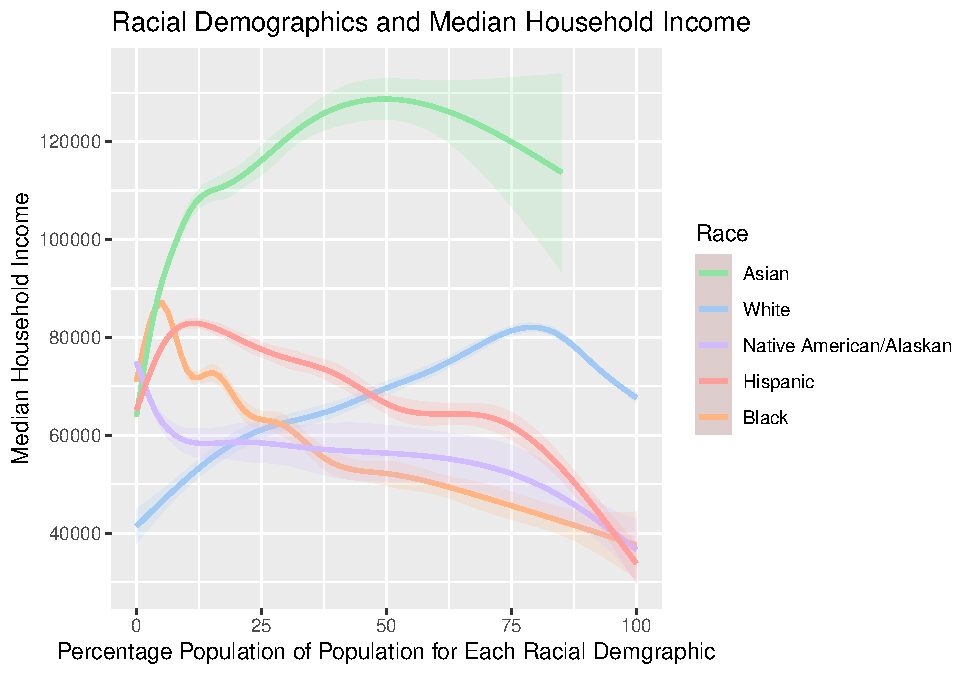
\includegraphics{Zip_Analysis_files/figure-latex/Smooth-Plot-Income-Race-1.pdf}
\caption{\label{fig:Smooth-Plot-Income-Race}Race-Income Plot}
\end{figure}

\begin{verbatim}
## Warning: Removed 3153 rows containing non-finite values (`stat_smooth()`).
## Removed 3153 rows containing non-finite values (`stat_smooth()`).
## Removed 3153 rows containing non-finite values (`stat_smooth()`).
## Removed 3153 rows containing non-finite values (`stat_smooth()`).
## Removed 3153 rows containing non-finite values (`stat_smooth()`).
\end{verbatim}

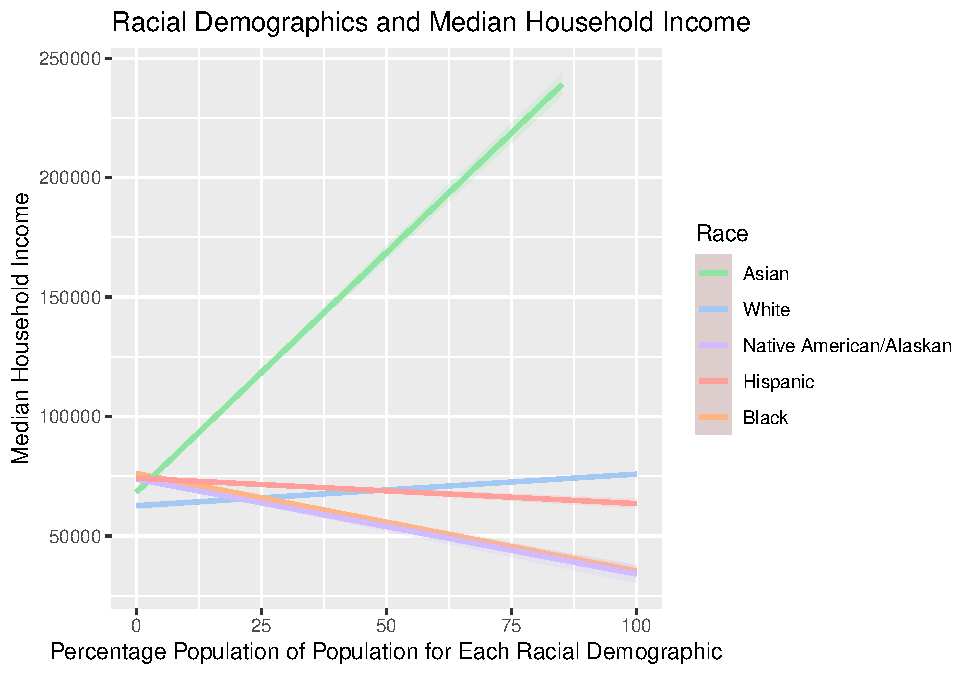
\includegraphics{Zip_Analysis_files/figure-latex/lm-plot-1.pdf}

\begin{verbatim}
## Warning: Removed 587 rows containing non-finite values (`stat_boxplot()`).
\end{verbatim}

\begin{figure}
\centering
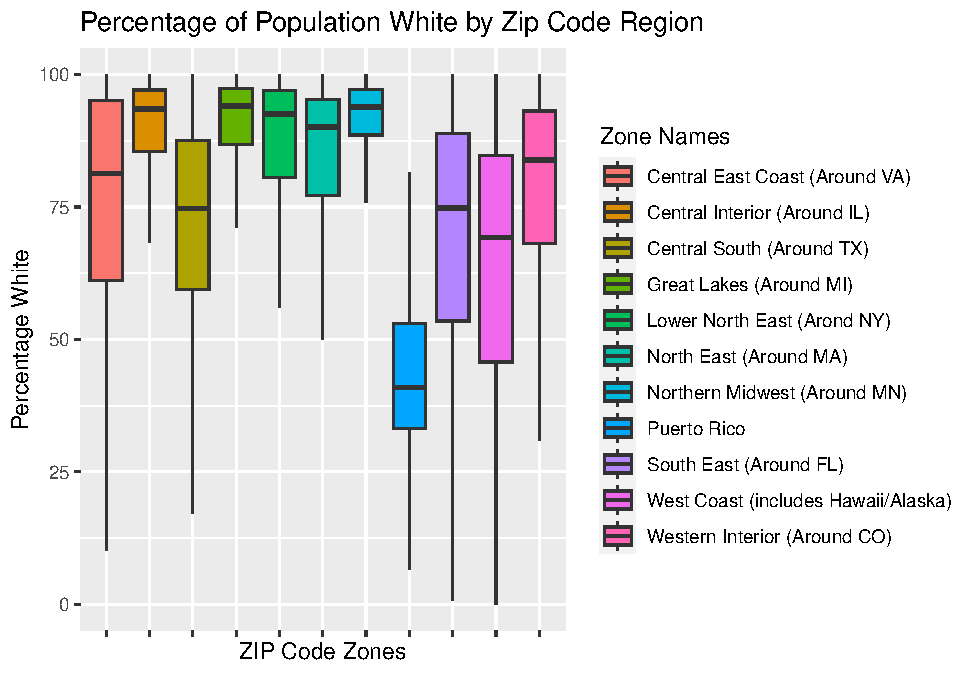
\includegraphics{Zip_Analysis_files/figure-latex/Whiteness-Income-Boxplot-1.pdf}
\caption{\label{fig:Whiteness-Income-Boxplot}(ref:Whiteness-Income-Boxplot-Caption)}
\end{figure}



\begin{table}

\caption{\label{tab:ZIP-Region-Table}Average ZIP Code Demographics by Region}
\resizebox{\ifdim\width>\linewidth\linewidth\else\width\fi}{!}{
\begin{tabular}[t]{l|>{}r|l|>{}r|l|>{}r|l|>{}r|l|>{}r|l|>{}r}
\hline
Region & \% White & SD White & \% Black & SD Black & \% Asian & SD Asian & \% Native Americn & SD Native American & \% Hispanic & SD Hispanic & ZIP Codes Per Region\\
\hline
Central East Coast (Around VA) & \textbf{75.02} & 23.79 & \textbf{15.97} & 20.58 & \textbf{1.85} & 4.47 & \textbf{0.53} & 3.80 & \textbf{5.47} & 7.66 & \textbf{3452}\\
\hline
Central Interior (Around IL) & \textbf{87.65} & 16.50 & \textbf{4.12} & 12.27 & \textbf{1.34} & 3.58 & \textbf{0.58} & 3.36 & \textbf{5.78} & 9.86 & \textbf{3721}\\
\hline
Central South (Around TX) & \textbf{71.48} & 20.73 & \textbf{11.12} & 17.71 & \textbf{1.62} & 3.89 & \textbf{2.05} & 5.32 & \textbf{19.83} & 24.46 & \textbf{3808}\\
\hline
Great Lakes (Around MI) & \textbf{88.36} & 16.24 & \textbf{5.32} & 13.45 & \textbf{1.05} & 2.67 & \textbf{0.32} & 1.56 & \textbf{3.47} & 5.70 & \textbf{3812}\\
\hline
Lower North East (Arond NY) & \textbf{84.84} & 19.50 & \textbf{5.30} & 12.05 & \textbf{2.59} & 6.03 & \textbf{0.29} & 2.54 & \textbf{6.36} & 10.47 & \textbf{3726}\\
\hline
North East (Around MA) & \textbf{83.01} & 18.66 & \textbf{4.39} & 9.62 & \textbf{3.95} & 7.19 & \textbf{0.32} & 1.56 & \textbf{8.06} & 12.45 & \textbf{2445}\\
\hline
Northern Midwest (Around MN) & \textbf{89.37} & 15.50 & \textbf{1.48} & 5.30 & \textbf{1.05} & 2.77 & \textbf{3.08} & 12.65 & \textbf{3.74} & 5.62 & \textbf{3766}\\
\hline
Puerto Rico & \textbf{43.15} & 18.15 & \textbf{9.12} & 9.05 & \textbf{0.23} & 0.45 & \textbf{0.15} & 0.26 & \textbf{97.96} & 6.07 & \textbf{132}\\
\hline
South East (Around FL) & \textbf{68.73} & 24.74 & \textbf{21.41} & 24.39 & \textbf{1.55} & 3.32 & \textbf{0.33} & 1.23 & \textbf{9.14} & 14.17 & \textbf{3483}\\
\hline
West Coast (includes Hawaii/Alaska) & \textbf{63.64} & 26.01 & \textbf{3.04} & 5.78 & \textbf{7.91} & 12.41 & \textbf{5.51} & 17.96 & \textbf{22.06} & 23.07 & \textbf{3177}\\
\hline
Western Interior (Around CO) & \textbf{76.22} & 24.31 & \textbf{1.77} & 4.17 & \textbf{1.43} & 2.87 & \textbf{6.29} & 20.06 & \textbf{20.39} & 23.04 & \textbf{2252}\\
\hline
\end{tabular}}
\end{table}

I will now refer to ``Figure~\ref{fig:Smooth-Plot-Income-Race}'' , Figure \ref{fig:Smooth-Plot-Income-Race}, Figure @ref(fig:Race-Income Plot), Figure~@ref(fig:Race-Income Plot)

Descriptive Chunk:

\begin{table}[tbp]

\begin{center}
\begin{threeparttable}

\caption{\label{tab:unnamed-chunk-2}}

\begin{tabular}{lllllll}
\toprule
measure & \multicolumn{1}{c}{mean} & \multicolumn{1}{c}{median} & \multicolumn{1}{c}{sd} & \multicolumn{1}{c}{first\_quartile} & \multicolumn{1}{c}{third\_quartile} & \multicolumn{1}{c}{range}\\
\midrule
Median\_Household\_Income & 73,132.63 & 66,993.00 & 31,359.58 & 53,466.00 & 85,313.00 & 247,502.00\\
X\_Total\_Population\_White\_Alone & 78.92 & 87.45 & 22.12 & 69.49 & 95.04 & 100.00\\
\bottomrule
\end{tabular}

\end{threeparttable}
\end{center}

\end{table}

Hypothesis Testing: Whiteness/Income

\begin{verbatim}
## [1] 0.09329494
\end{verbatim}

\begin{verbatim}
## [1] 3.656746e-60
\end{verbatim}

\begin{verbatim}
## Warning: Removed 3153 rows containing non-finite values (`stat_smooth()`).
\end{verbatim}

\begin{verbatim}
## Warning: Removed 3153 rows containing missing values (`geom_point()`).
\end{verbatim}

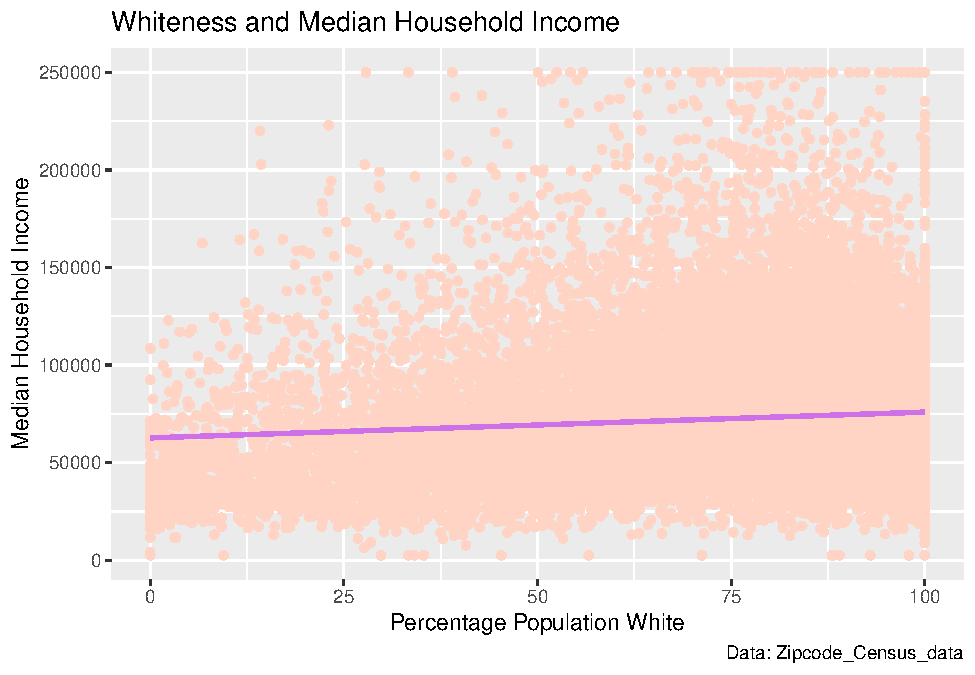
\includegraphics{Zip_Analysis_files/figure-latex/whiteness-income-plot-1.pdf}

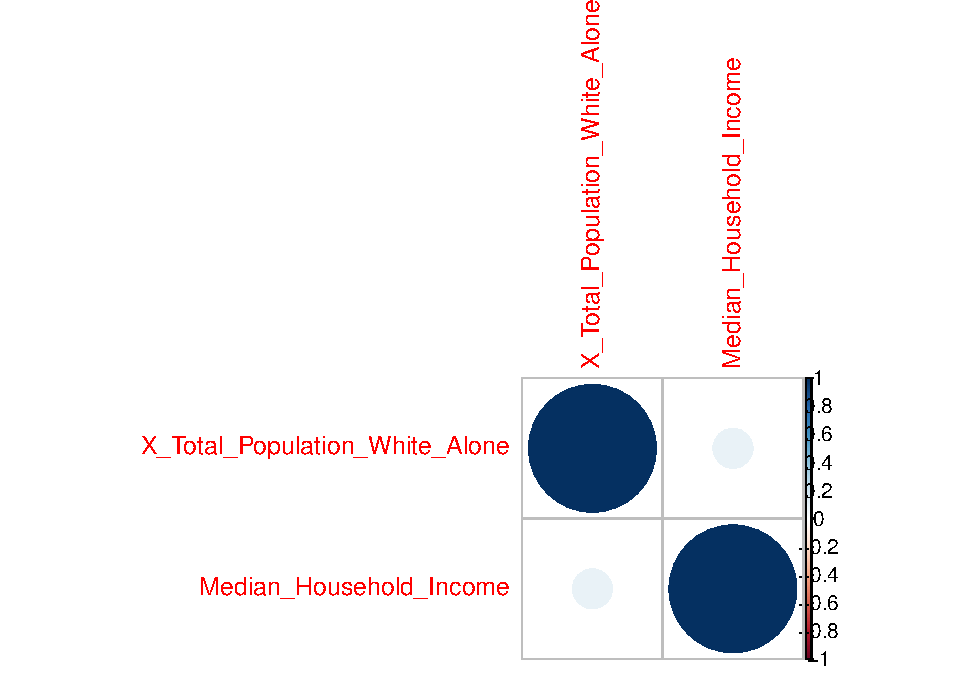
\includegraphics{Zip_Analysis_files/figure-latex/unnamed-chunk-3-1.pdf}

\begin{verbatim}
## 
##  Welch Two Sample t-test
## 
## data:  filter(Census_desc2, X_Total_Population_White_Alone >= 75)$Median_Household_Income and filter(Census_desc2, X_Total_Population_White_Alone <= 75)$Median_Household_Income
## t = 10.021, df = 15398, p-value < 2.2e-16
## alternative hypothesis: true difference in means is not equal to 0
## 95 percent confidence interval:
##  3348.951 4977.716
## sample estimates:
## mean of x mean of y 
##  74406.65  70243.32
\end{verbatim}

\begin{verbatim}
## 
##  Welch Two Sample t-test
## 
## data:  filter(Census_desc2, X_Total_Population_Asian_Alone >= 50, Zipcode_Zone == "West Coast (includes Hawaii/Alaska)")$Median_Household_Income and filter(Census_desc2, X_Total_Population_White_Alone <= 50, Zipcode_Zone == "West Coast (includes Hawaii/Alaska)")$Median_Household_Income
## t = 7.547, df = 70.625, p-value = 1.187e-10
## alternative hypothesis: true difference in means is not equal to 0
## 95 percent confidence interval:
##  35308.15 60667.43
## sample estimates:
## mean of x mean of y 
##  130621.3   82633.5
\end{verbatim}

\hypertarget{results}{%
\section{Results}\label{results}}

\hypertarget{discussion}{%
\section{Discussion}\label{discussion}}

\newpage

\hypertarget{references}{%
\section{References}\label{references}}

\hypertarget{refs}{}
\begin{CSLReferences}{0}{0}
\end{CSLReferences}


\end{document}
